\documentclass[11pt,a4paper]{article}

\usepackage[utf8]{inputenc}
\usepackage[T1]{fontenc}
\usepackage{lmodern}
\usepackage{geometry}
\geometry{a4paper, margin=2.4cm}
\usepackage{microtype}
\usepackage{graphicx}
\usepackage{booktabs}
\usepackage{siunitx}
\usepackage{xcolor}
\usepackage{amsmath}
\usepackage{amssymb}
\usepackage[hidelinks]{hyperref}
\usepackage{cleveref}
\usepackage{enumitem}
\usepackage{caption}
\captionsetup{labelfont=bf,font=small}
\usepackage{listings}
\usepackage{tcolorbox}
\tcbuselibrary{listings, skins, breakable}
\usepackage{titlesec}
\usepackage{parskip}
\usepackage{fancyhdr}

\definecolor{codebg}{HTML}{F6F8FA}
\definecolor{codeframe}{HTML}{D0D7DE}
\definecolor{kw}{HTML}{0550AE}
\definecolor{str}{HTML}{0A3069}
\definecolor{cmt}{HTML}{6E7781}

\lstdefinelanguage{starfoldpy}[]{Python}{
  keywordstyle=\color{kw}\bfseries,
  stringstyle=\color{str},
  commentstyle=\color{cmt}\itshape,
  basicstyle=\ttfamily\footnotesize,
  showstringspaces=false,
  breaklines=true,
  columns=fullflexible,
  upquote=true,
}

\newtcblisting{pycode}{
  listing only,
  listing options={language=starfoldpy},
  colback=codebg, colframe=codeframe,
  arc=2pt, boxrule=0.5pt,
  left=8pt, right=8pt, top=4pt, bottom=4pt,
  breakable,
}

\newtcolorbox{notebox}[1][]{
  colback=codebg, colframe=codeframe,
  arc=2pt, boxrule=0.5pt,
  left=8pt, right=8pt, top=4pt, bottom=4pt,
  fonttitle=\bfseries,
  #1
}

\titleformat{\section}{\Large\bfseries}{\thesection}{0.6em}{}
\titleformat{\subsection}{\large\bfseries}{\thesubsection}{0.6em}{}
\titleformat{\subsubsection}{\normalsize\bfseries}{\thesubsubsection}{0.6em}{}

\pagestyle{fancy}
\fancyhf{}
\fancyhead[L]{\small\textsc{starfold}}
\fancyhead[R]{\small\thepage}
\renewcommand{\headrulewidth}{0.3pt}

\graphicspath{{figures/tutorial_00_walkthrough/}{figures/tutorial_01_quickstart/}{figures/tutorial_02_validation/}{figures/tutorial_03_advanced/}{figures/tutorial_04_astronomy/}}

\title{\textbf{\textsf{starfold}}\\[0.4em]
       \large A domain-agnostic UMAP+HDBSCAN clustering pipeline with statistical reliability quantification}
\author{Andreas W. Neitzel\\
        \small Instituto de Astrofísica e Ciências do Espaço, Universidade do Porto\\
        \small \href{https://orcid.org/0000-0001-6283-907X}{ORCID 0000-0001-6283-907X}}
\date{Documentation, May 2026 (package version 0.0.1)}

\begin{document}
\maketitle

\begin{abstract}
\noindent
\textsf{starfold} packages a four-step unsupervised clustering pipeline as a single primitive, \texttt{UnsupervisedPipeline.fit(X)}, returning one immutable result dataclass, \texttt{PipelineResult}, that owns the full audit trail of the run. The core methodology follows §3 of Neitzel et al.\ 2025: \texttt{StandardScaler} $\rightarrow$ UMAP $\rightarrow$ Optuna-tuned HDBSCAN $\rightarrow$ trustworthiness, continuity, and a 99.7th-percentile noise baseline. On top of that core, the package ships a small set of paper-silent extensions that compose with the result object: a global 3-sigma credibility test, two modes of input-uncertainty propagation, a hierarchical merge recommender, and chunked-silhouette plus subsample-stability diagnostics. This document is the long-form reference: scope, installation, the public API surface (\num{30} symbols), every methodological choice with citations where the paper is silent, and worked examples with images at every step.
\end{abstract}

\tableofcontents
\vspace{1em}

% =========================================================================
\section{Scope and design}
\label{sec:scope}

\textsf{starfold} commits to one pipeline shape and exposes it as a single primitive. The package has two concentric scope rings:

\paragraph{Core (paper §3 fidelity).} The four-step pipeline implements Neitzel et al.\ (2025) §3 verbatim. Hyperparameter defaults and statistical thresholds match the paper exactly. This ring is non-negotiable.

\paragraph{Extensions (paper-silent, intentional).} On top of the core, \textsf{starfold} ships a small set of validation and refinement primitives that compose with \texttt{PipelineResult}: a global credibility test, input-uncertainty propagation, hierarchical refinement, robustness diagnostics, and sample-size-aware defaults. Extensions exist because the paper's per-cluster threshold and post-hoc workflow leave concrete user questions unanswered.

\paragraph{What the tool is not.} It is not a reproduction of the Neitzel et al.\ (2025) astronomical application. It does not construct stellar samples, apply survey selection functions, or know anything about galactic archaeology. It is not a general-purpose clustering toolkit either: users who want a different pipeline shape should compose \texttt{scikit-learn} directly.

\subsection{The two load-bearing primitives}

\begin{itemize}[leftmargin=*]
  \item \texttt{UnsupervisedPipeline} is the pipeline object. Configure it with UMAP and Optuna kwargs at construction time; call \texttt{.fit(X)} once.
  \item \texttt{PipelineResult} is the immutable result dataclass: 2-D embedding, integer cluster labels, per-cluster persistence, trustworthiness, continuity, the noise-baseline summary, the credibility report, the fitted scaler and reducer, the Optuna study, and the run configuration. All post-fit operations are methods on this object or free functions that take it.
\end{itemize}

% =========================================================================
\section{Installation}

\textsf{starfold} is not yet on PyPI. Install from GitHub:

\begin{pycode}
# pip
pip install "git+https://github.com/AndreasWNeitzel/starfold.git"

# uv (recommended)
uv add "git+https://github.com/AndreasWNeitzel/starfold.git"
\end{pycode}

Runtime dependencies: \texttt{numpy}, \texttt{scipy}, \texttt{scikit-learn}, \texttt{umap-learn}, \texttt{hdbscan}, \texttt{optuna}, \texttt{matplotlib}, \texttt{platformdirs}, \texttt{joblib}, \texttt{tqdm}. Python 3.11 or 3.12. An optional GPU backend via \texttt{cuml} is auto-detected when present.

% =========================================================================
\section{Quick start}
\label{sec:quickstart}

Any 2-D \texttt{numpy} array goes in; one fit comes out.

\begin{pycode}
import numpy as np
import starfold as sf

# X: (n_samples, n_features) numerical matrix. That's all this tool needs.
X = np.random.default_rng(0).normal(size=(3000, 5))

pipeline = sf.UnsupervisedPipeline(
    umap_kwargs={"n_neighbors": 15, "min_dist": 0.0},
    hdbscan_optuna_trials=100,
    random_state=42,
)
result = pipeline.fit(X)

result.embedding         # (n_samples, 2) float array
result.labels            # (n_samples,) int array, -1 for outliers
result.persistence       # (n_clusters,) float array
result.significant       # (n_clusters,) bool array vs noise baseline
result.trustworthiness   # float in [0, 1]
print(result.summary())  # printable metrics table
result.plot_embedding()  # colour-coded by label
result.save("run_01/")   # disk snapshot
\end{pycode}

\Cref{fig:quickstart-embedding} shows the result on \textsf{sklearn}'s \texttt{digits} dataset (1\,797 samples, 64 features, 10 true classes). The pipeline recovers the digit classes with no supervision.

\begin{figure}[h]
  \centering
  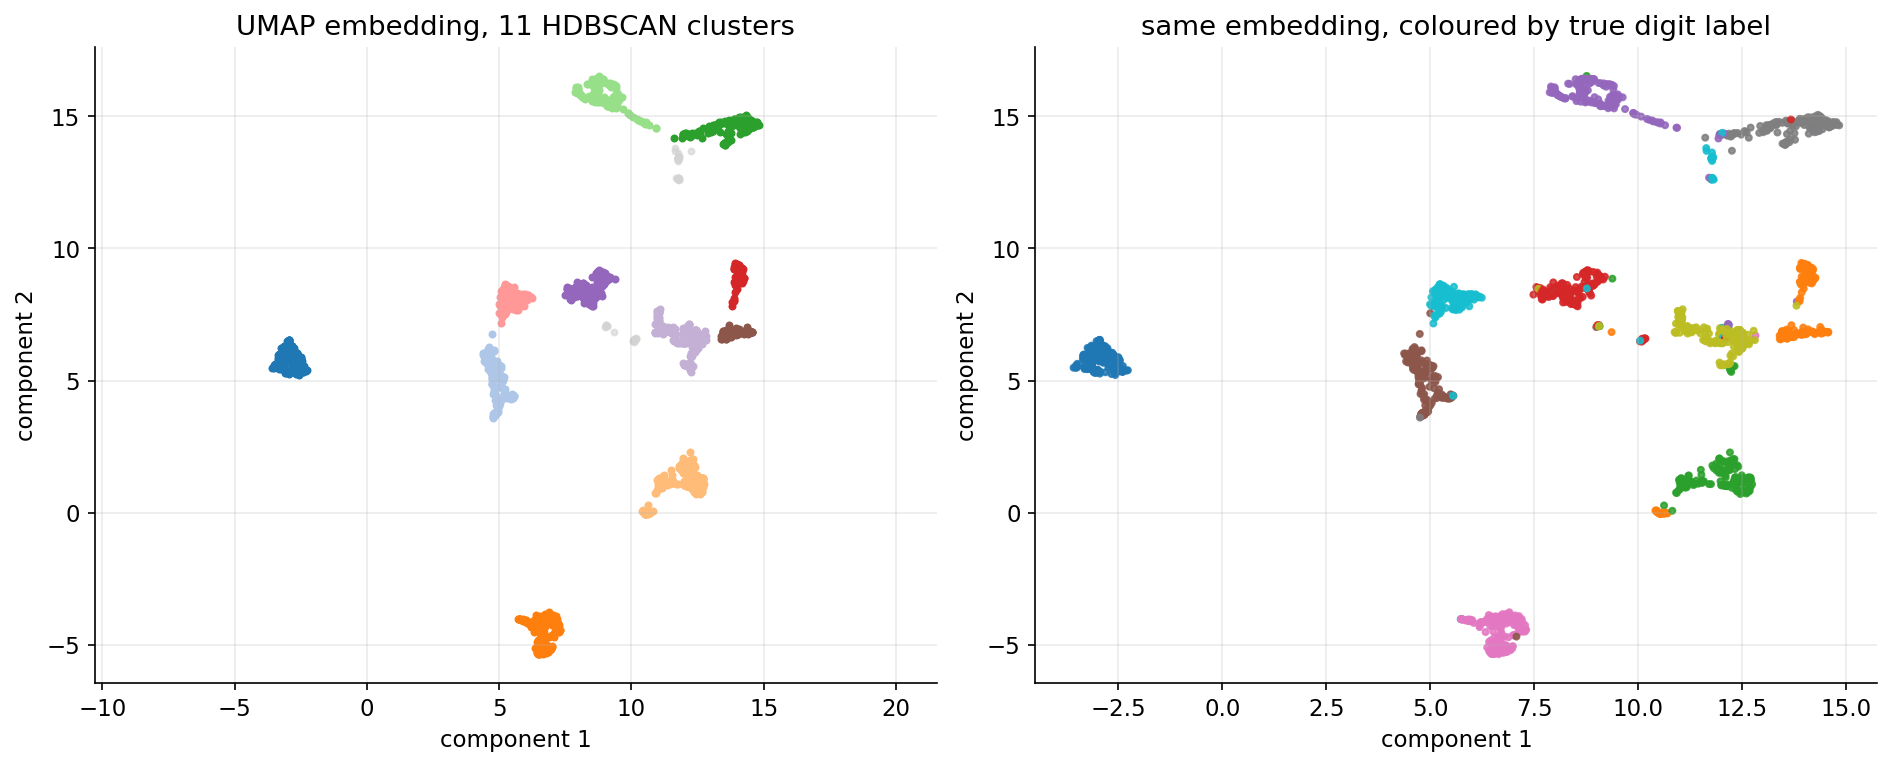
\includegraphics[width=0.85\textwidth]{02_pipeline_embedding.png}
  \caption{Quickstart output on the \texttt{sklearn.datasets.load\_digits} dataset: 2-D UMAP embedding coloured by HDBSCAN cluster, outliers in grey. The unsupervised pipeline recovers structure that corresponds closely to the ten true digit classes.}
  \label{fig:quickstart-embedding}
\end{figure}

% =========================================================================
\section{The core pipeline}
\label{sec:core}

\subsection{What \texttt{fit} does, step by step}

A single \texttt{pipeline.fit(X)} call runs the four-step pipeline in order:

\begin{enumerate}[leftmargin=*]
  \item \textbf{Standardisation.} \texttt{StandardScaler} fits and transforms \(X\) so every feature has zero mean and unit variance. The scaler is stored on the result for reproducibility.
  \item \textbf{UMAP embedding.} A 2-D UMAP embedding with \texttt{n\_neighbors=15}, \texttt{min\_dist=0.0}, \texttt{n\_epochs=10\,000} by default (paper §3.1). \texttt{random\_state} propagates.
  \item \textbf{Optuna-tuned HDBSCAN.} An Optuna TPE search over \texttt{min\_cluster\_size} (log-uniform integer in \([5, 500]\)) and \texttt{min\_samples} (log-uniform in \([1, 50]\)) maximises the sum of \texttt{cluster\_persistence\_} across returned clusters. Default budget: 100 trials.
  \item \textbf{Trustworthiness, continuity, and noise baseline.} Trustworthiness (Venna and Kaski 2001) and its complementary continuity score at \(k = \texttt{n\_neighbors}\) are computed against \texttt{sklearn}'s reference implementation at \(\mathrm{atol} = 10^{-10}\). The 99.7th-percentile noise baseline is computed from \num{1000} Gaussian noise realisations; each cluster is flagged \texttt{significant} iff its persistence exceeds the threshold.
\end{enumerate}

\subsection{What lives on \texttt{PipelineResult}}

Beyond the headline arrays listed in \Cref{sec:quickstart}, the result carries the Optuna \texttt{study} (for hyperparameter inspection), the fitted UMAP \texttt{reducer}, the noise-baseline summary, the optional credibility report, and a \texttt{flags} list of diagnostic warnings. Methods on the result:

\begin{itemize}[leftmargin=*,nosep]
  \item \texttt{.summary()} \(\rightarrow\) printable metrics table.
  \item \texttt{.silhouette(chunk\_size=512)} \(\rightarrow\) chunked silhouette result (per cluster + global, memory-efficient).
  \item \texttt{.suggest\_merges()} \(\rightarrow\) cluster-pair merge recommendations from the condensed tree.
  \item \texttt{.refit\_subcluster(X, cluster\_id)} \(\rightarrow\) second-pass fit on a subset.
  \item \texttt{.propagate\_uncertainty(X, sigma, n\_draws)} \(\rightarrow\) post-hoc Monte Carlo propagation.
  \item \texttt{.plot\_tuning\_dashboard()}, \texttt{.plot\_quality\_dashboard(X)} \(\rightarrow\) the two one-call dashboards.
  \item \texttt{.save(path)} \(\rightarrow\) disk snapshot.
\end{itemize}

\subsection{Why UMAP beats t-SNE and PCA for this pipeline}

\Cref{fig:embedding-comparison} shows \texttt{run\_umap}, \texttt{run\_tsne}, and \texttt{run\_pca} on the same digits data. UMAP delivers the cleanest cluster separation; t-SNE produces visible clusters but with weaker inter-cluster gaps; PCA cannot disentangle the manifold and produces overlapping blobs. The pipeline is built around UMAP, but the alternatives are exposed as standalone helpers for comparison plots.

\begin{figure}[h]
  \centering
  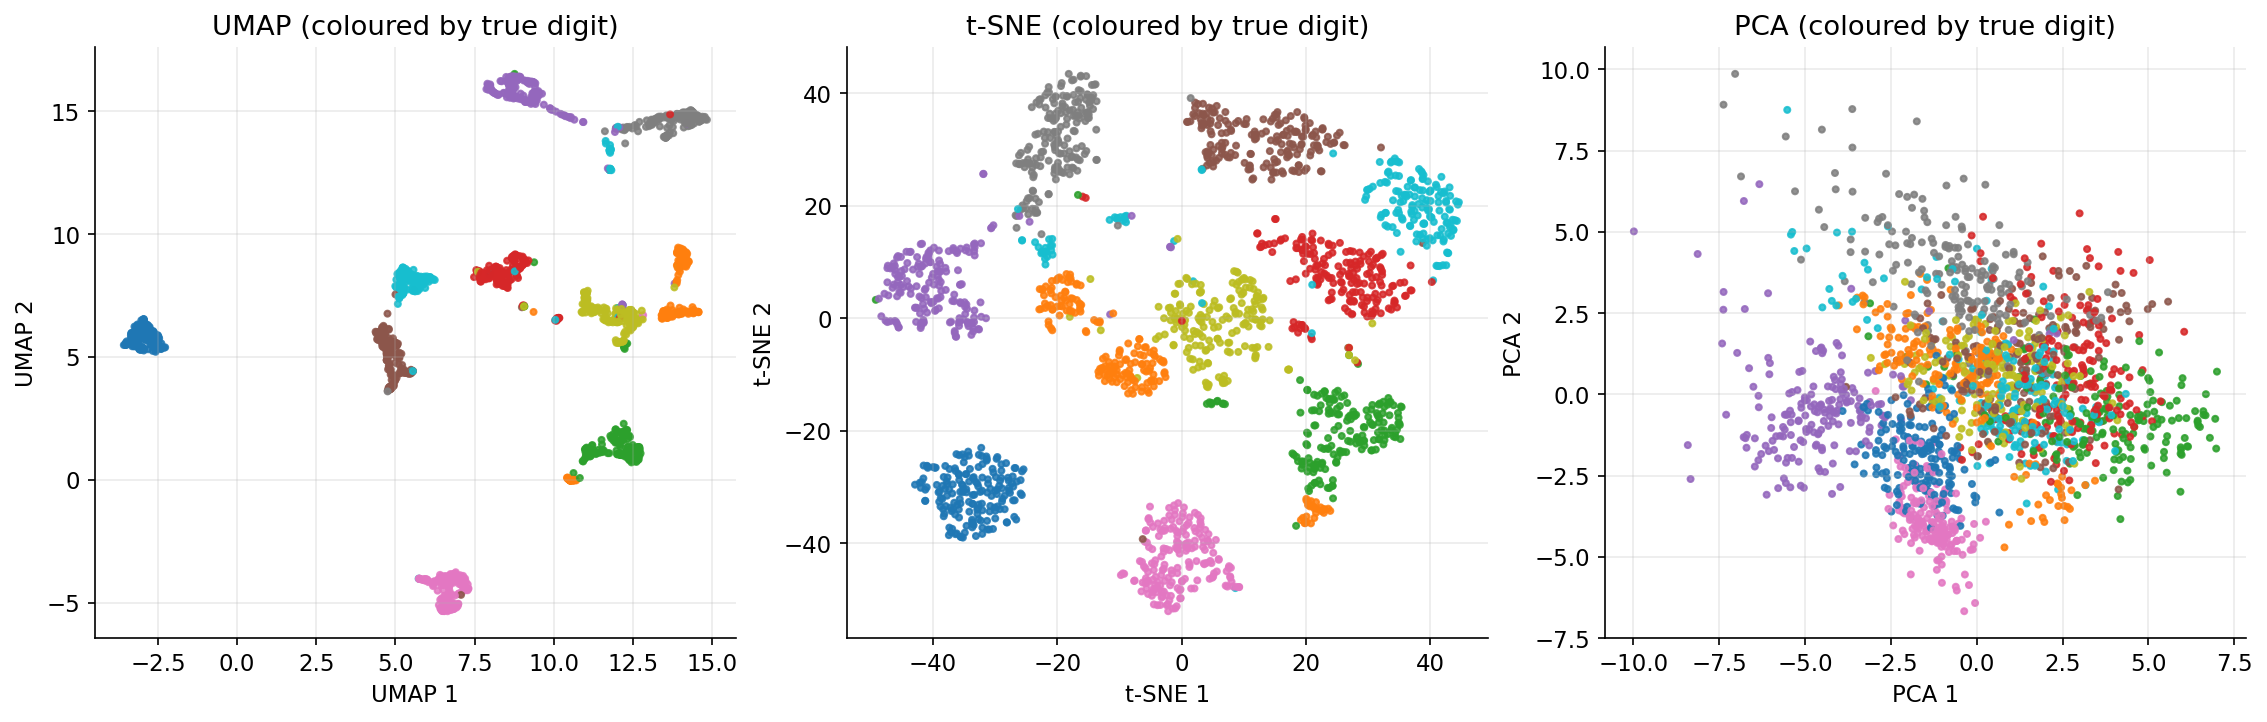
\includegraphics[width=\textwidth]{03_embedding_comparison.png}
  \caption{2-D embeddings of the digits data produced by UMAP, t-SNE, and PCA. UMAP recovers the clearest cluster separation; PCA cannot.}
  \label{fig:embedding-comparison}
\end{figure}

% =========================================================================
\section{Methodology}
\label{sec:methodology}

This section explains each pipeline step and the paper-silent design choices in detail.

\subsection{UMAP (§3.1)}

UMAP defaults follow the paper: \texttt{n\_neighbors=15}, \texttt{min\_dist=0.0}, \texttt{n\_epochs=10\,000}. The paper notes convergence by \(\sim 1000\) epochs; we keep \num{10000} as a default safety margin. The input must be pre-standardised by the caller. \texttt{UnsupervisedPipeline} does this internally with \texttt{StandardScaler}; \texttt{run\_umap} on its own does not (it is a thin wrapper).

\subsection{Trustworthiness and continuity (§3.2)}

The trustworthiness score (Venna and Kaski 2001) penalises false neighbours in the embedding:
\begin{equation}
  T(k) = 1 - \frac{2}{N k (2N - 3k - 1)} \sum_{i=1}^{N} \sum_{x_j \in U_k(x_i)} \left( r(x_i, x_j) - k \right),
\end{equation}
where \(U_k(x_i)\) is the set of \(k\) nearest neighbours of \(x_i\) in the embedding that are not \(k\) nearest neighbours of \(x_i\) in the input, and \(r(x_i, x_j)\) is the rank of \(x_j\) ordered by distance to \(x_i\) in the input. Continuity is the symmetric measure (false missing neighbours). \textsf{starfold}'s implementation is cross-tested against \texttt{sklearn.manifold.trustworthiness} at \(\mathrm{atol} = 10^{-10}\) across five seeded datasets covering \(N \in \{100, 500, 2000, 5000\}\) and \(k \in \{5, 15, 30\}\).

The paper's acceptance heuristic is \(T(k = \texttt{n\_neighbors}) > 0.90\). \textsf{starfold} reports the value but does not hardcode the threshold.

\subsection{HDBSCAN and Optuna (§3.3)}

Clustering: \texttt{hdbscan.HDBSCAN(min\_cluster\_size, min\_samples, gen\_min\_span\_tree=True)}. The objective is the sum (not the max) of \texttt{cluster\_persistence\_} across returned clusters, so the search rewards both more clusters and more persistent ones.

\paragraph{Search space (paper-silent, our choice).} \texttt{min\_cluster\_size} log-uniform integer in \([5, 500]\); on samples where \(n / 10 < 500\) the upper bound is capped to \(\max(5, n/10)\) via \texttt{auto\_mcs\_upper}. \texttt{min\_samples} log-uniform integer in \([1, 50]\). Sampler: \texttt{optuna.samplers.TPESampler(seed=random\_state)}. No pruner.

\subsection{Noise baseline (§3.3)}

The reliability baseline answers ``would Gaussian noise of the same shape produce clusters this persistent?''. The procedure:

\begin{enumerate}[leftmargin=*,nosep]
  \item Draw \texttt{n\_realisations} (default \num{1000}) Gaussian matrices of shape \((n, p)\).
  \item For each, run UMAP with the user's \texttt{umap\_kwargs}, then Optuna+HDBSCAN with \texttt{per\_realisation\_trials} (default 20). Record the max cluster persistence.
  \item The 99.7th-percentile (3-sigma) of those maxima is the threshold. Each real cluster's \texttt{significant} flag is \texttt{persistence > threshold}.
\end{enumerate}

The result is cached on disk under \texttt{platformdirs.user\_cache\_dir("starfold")}, keyed on a hash of \((n, p, \text{frozen umap\_kwargs}, \text{random\_state}, \text{n\_realisations}, \text{per\_realisation\_trials})\). \Cref{fig:persistence-vs-baseline} shows the typical output of the baseline on a clean dataset.

\begin{figure}[h]
  \centering
  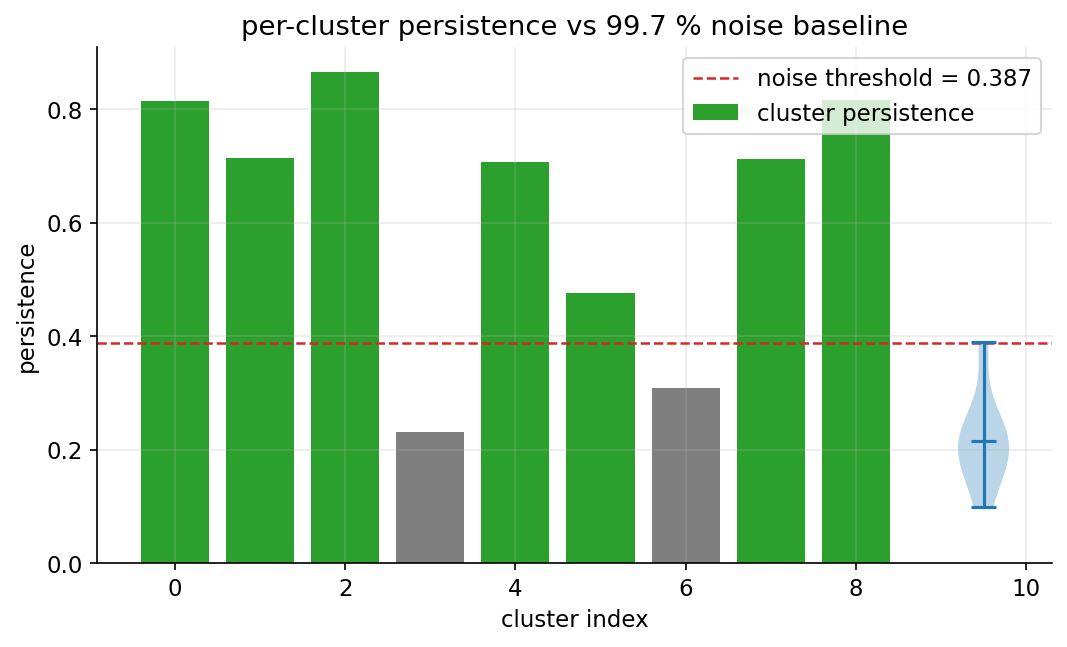
\includegraphics[width=0.85\textwidth]{01_persistence_vs_baseline.png}
  \caption{Per-cluster persistence (bars) against the 99.7th-percentile noise baseline (dashed line). Clusters above the line are flagged \texttt{significant}; the cluster on the right falls just under threshold.}
  \label{fig:persistence-vs-baseline}
\end{figure}

\subsection{The omnibus 3-sigma credibility test}
\label{sec:credibility}

The per-cluster significance flag answers ``is this cluster real?''. A separate question is ``is the whole run distinguishable from noise?''. \texttt{compute\_credibility} aggregates three per-run scalars against the noise null:
\begin{itemize}[leftmargin=*,nosep]
  \item \texttt{n\_clusters} (count of clusters returned).
  \item \texttt{best\_objective} (Optuna's best persistence sum).
  \item \texttt{max\_persistence} (single strongest cluster).
\end{itemize}
Each scalar has a one-sided upper-tail empirical p-value with the Phipson and Smyth (2010) \((r+1)/(n+1)\) correction (so a p-value is never exactly zero). The run \texttt{passes} at 3-sigma when all three p-values clear \(\alpha = 0.003\). The credibility report is \texttt{result.credibility}; \Cref{fig:credibility} shows the canonical three-panel visual.

\begin{figure}[h]
  \centering
  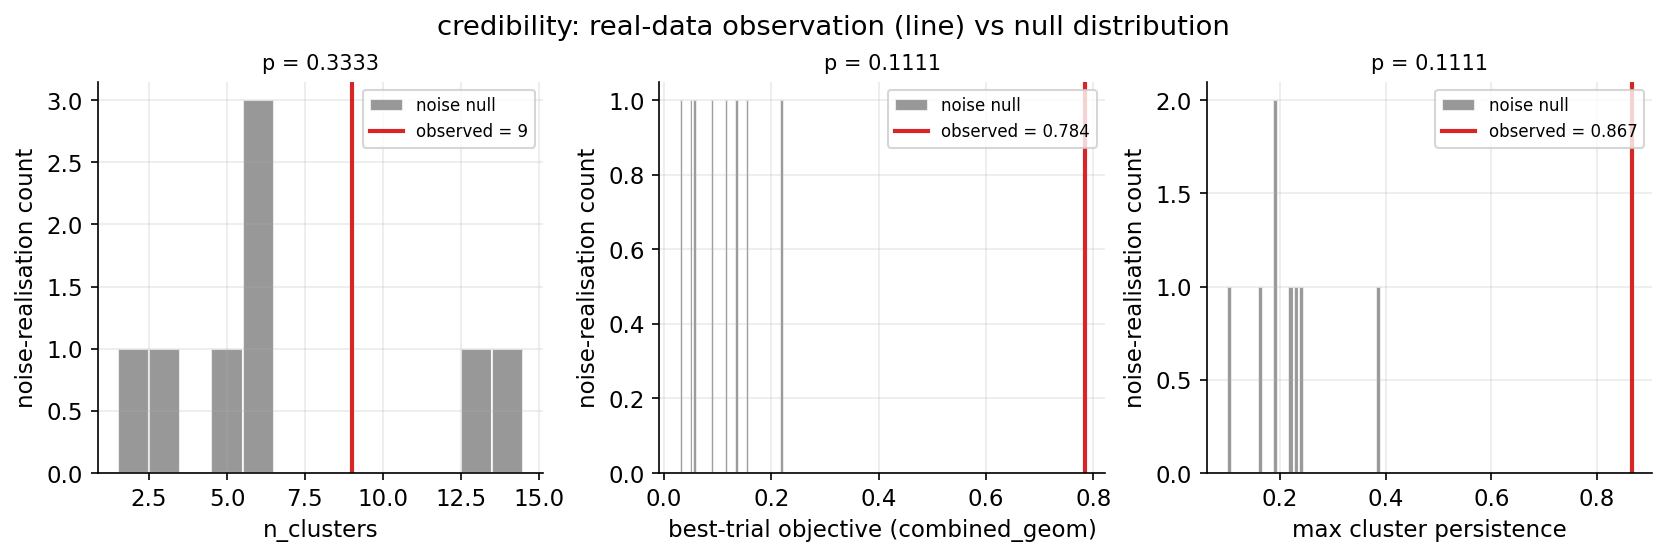
\includegraphics[width=\textwidth]{02_credibility_three_axes.png}
  \caption{Credibility report: each scalar (top to bottom: cluster count, best objective, max persistence) plotted against its empirical null distribution from the noise realisations. The observed value (vertical line) lands in the upper tail in each case; the omnibus p-value clears 3-sigma.}
  \label{fig:credibility}
\end{figure}

% =========================================================================
\section{Extensions}
\label{sec:extensions}

\subsection{Input-uncertainty propagation}
\label{sec:uncertainty}

When the user's feature matrix carries per-feature 1-sigma error bars, \textsf{starfold} can propagate that uncertainty into a per-sample probability distribution over cluster identities. Two modes:

\paragraph{Mode A: post-hoc Monte Carlo.}
\texttt{result.propagate\_uncertainty(X, sigma, n\_draws)} freezes the fitted UMAP and HDBSCAN models, draws \texttt{n\_draws} perturbations of \(X\) from \(\mathcal{N}(X, \sigma)\) (with \texttt{sigma} a scalar, a 1-D vector, or a 2-D \((n, p)\) matrix), and assigns each replica via \texttt{umap.transform} + \texttt{hdbscan.approximate\_predict}. The output \texttt{UncertaintyPropagation} dataclass exposes \texttt{membership} of shape \((n, K + 1)\), where \texttt{membership[i, k]} is the fraction of draws in which sample \(i\) landed in cluster \(k\) (column \(K\) is the outlier fraction), plus \texttt{instability \(= 1 - \max_k \texttt{membership}[i, k]\)}.

\paragraph{Mode B: uncertainty-aware fit.}
\texttt{pipeline.fit\_with\_uncertainty(X, sigma, n\_replicas)} stacks \(\texttt{n\_replicas}\) Gaussian-perturbed copies of \(X\) on top of the clean matrix and runs the full pipeline on the augmented \((1 + \texttt{n\_replicas}) \cdot n\) row matrix. UMAP and HDBSCAN see the spread itself, so the noise baseline and credibility are computed against the enlarged sample. The returned \texttt{UncertaintyAwareFit} bundles the augmented \texttt{PipelineResult} with a per-original-sample \texttt{UncertaintyPropagation}.

\paragraph{The two modes answer different questions.}
Mode A audits an existing clustering: ``given this fit, how stable is each label?''. Mode B renegotiates the clustering itself: ``what structure does the data support when its uncertainty cloud is part of the fitting input?''. The two can disagree directionally and that disagreement is itself a reliability signal.

\paragraph{A topology-stress demonstration.} Well-separated blobs are not a good test of uncertainty propagation: as long as sigma stays smaller than the inter-cluster gap, the membership matrix is near one-hot. A closed chain of four Hopf-linked tori (\Cref{fig:torus-truth}) is the natural stress test: adjacent rings thread each other's holes, so they share a boundary region that uncertainty can blur.

\begin{figure}[h]
  \centering
  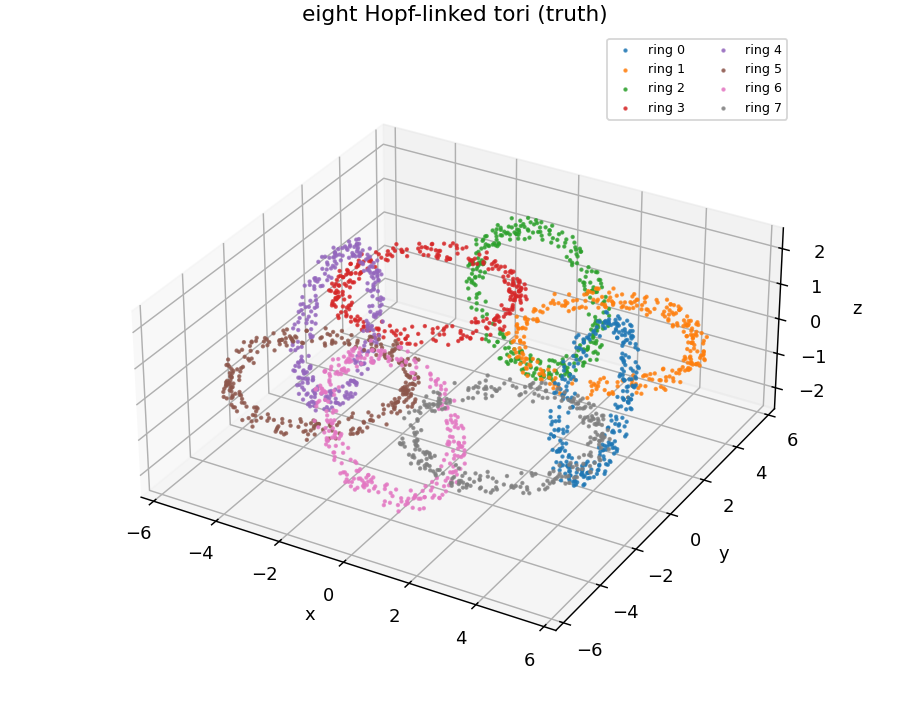
\includegraphics[width=0.65\textwidth]{13_torus_chain_truth.png}
  \caption{Four-torus closed Hopf chain in 3D. Adjacent rings link; non-adjacent rings do not. Augmented with two heteroscedastic ``metadata'' features to make the pipeline see a 5-D feature matrix.}
  \label{fig:torus-truth}
\end{figure}

Running \texttt{propagate\_uncertainty} at three sigma scales (\(\times 1\), \(\times 5\), \(\times 15\) of a baseline per-feature vector) produces a controlled breakdown (\Cref{fig:torus-sweep}):

\begin{table}[h]
  \centering
  \caption{Reliability under growing per-feature uncertainty on the four-torus chain.}
  \label{tab:sigma-sweep}
  \begin{tabular}{rrrr}
    \toprule
    sigma & mean instability & confident (\(<0.1\)) & high-doubt (\(>0.5\)) \\
    \midrule
    \(\times 1.0\)  & 0.011 & 96.4\% & 0.0\% \\
    \(\times 5.0\)  & 0.070 & 79.5\% & small \\
    \(\times 15.0\) & 0.317 & 19.4\% & substantial \\
    \bottomrule
  \end{tabular}
\end{table}

\begin{figure}[h]
  \centering
  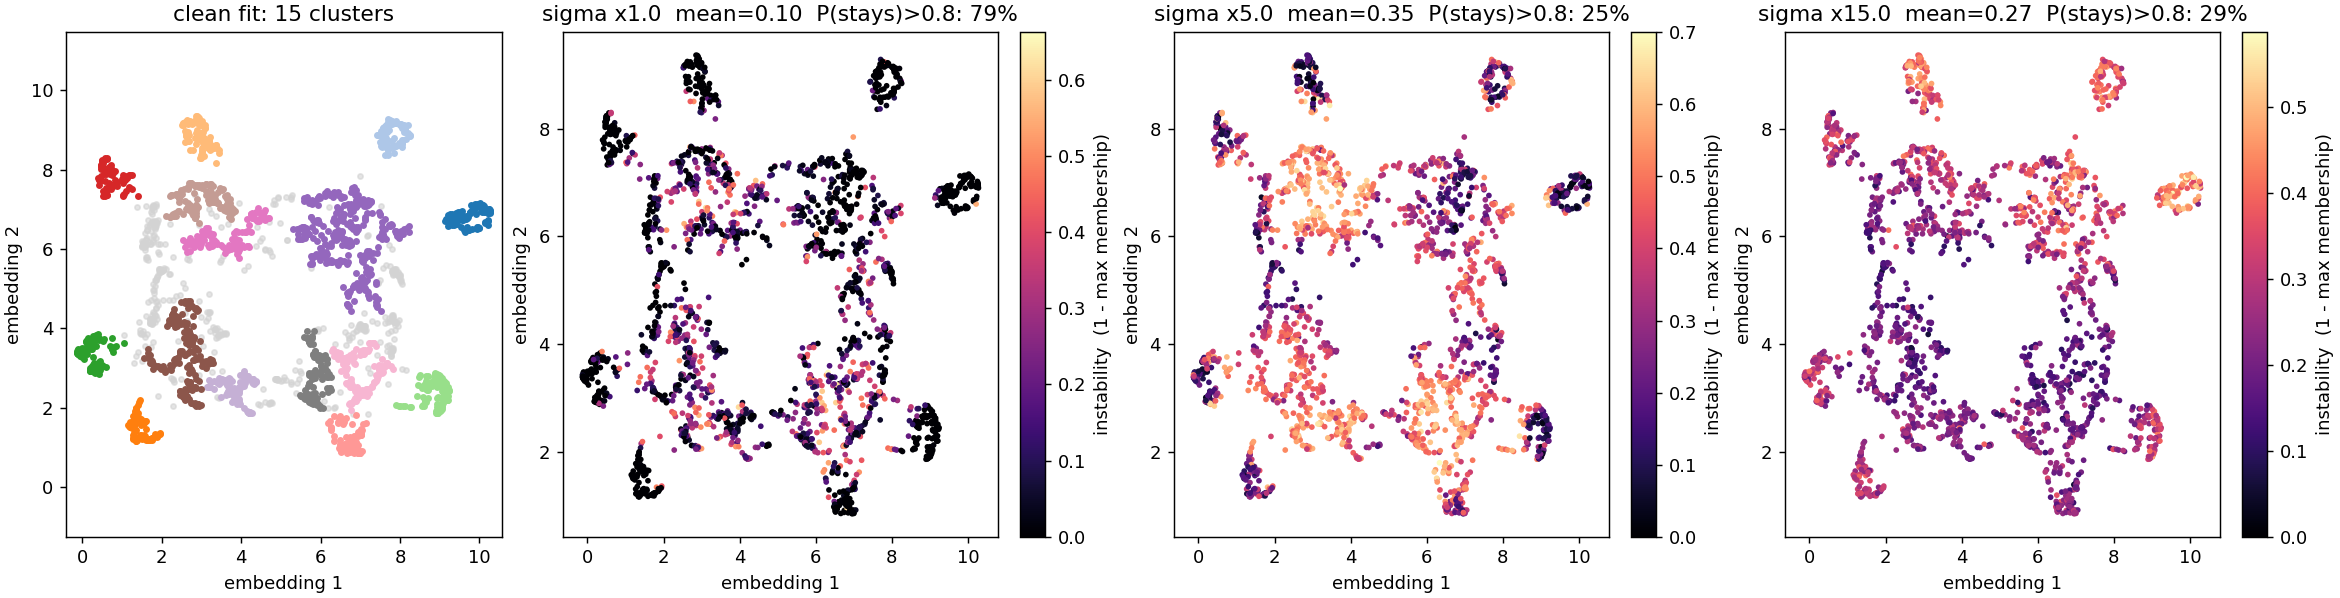
\includegraphics[width=\textwidth]{14_torus_uncertainty_sweep.png}
  \caption{Topology stress test. Left: clean fit embedding coloured by HDBSCAN label. Right three panels: instability map at growing sigma. Bright regions concentrate at the link points between adjacent rings, then engulf entire rings.}
  \label{fig:torus-sweep}
\end{figure}

At \(\times 15\) a single boundary sample's membership row reads \(P(c_2) = 0.28,\ P(c_3) = 0.26,\ P(c_4) = 0.25,\ P(\mathrm{out}) = 0.20\): assignment is essentially uniform across three adjacent rings plus the outlier column. This is the quantitative reliability statement the user can report alongside the hard label.

\subsection{Hierarchical refinement: \texttt{suggest\_merges}}
\label{sec:merges}

After a clean fit, you may suspect HDBSCAN over-split one true cluster into two. \texttt{result.suggest\_merges()} walks the condensed-tree structure and flags candidate pairs where two clusters are both
\begin{itemize}[leftmargin=*,nosep]
  \item \textbf{cohesive} in density (sibling branches in the tree, high \texttt{cohesion\_ratio}), and
  \item \textbf{geometrically close} in the embedding (\texttt{gap\_ratio} below threshold).
\end{itemize}
A merge is \texttt{recommended} when both conditions clear default thresholds (cohesion \(\geq 0.9\), gap \(\leq 2.0\)). \Cref{fig:merge-candidates} shows the recommendation panel.

\begin{figure}[h]
  \centering
  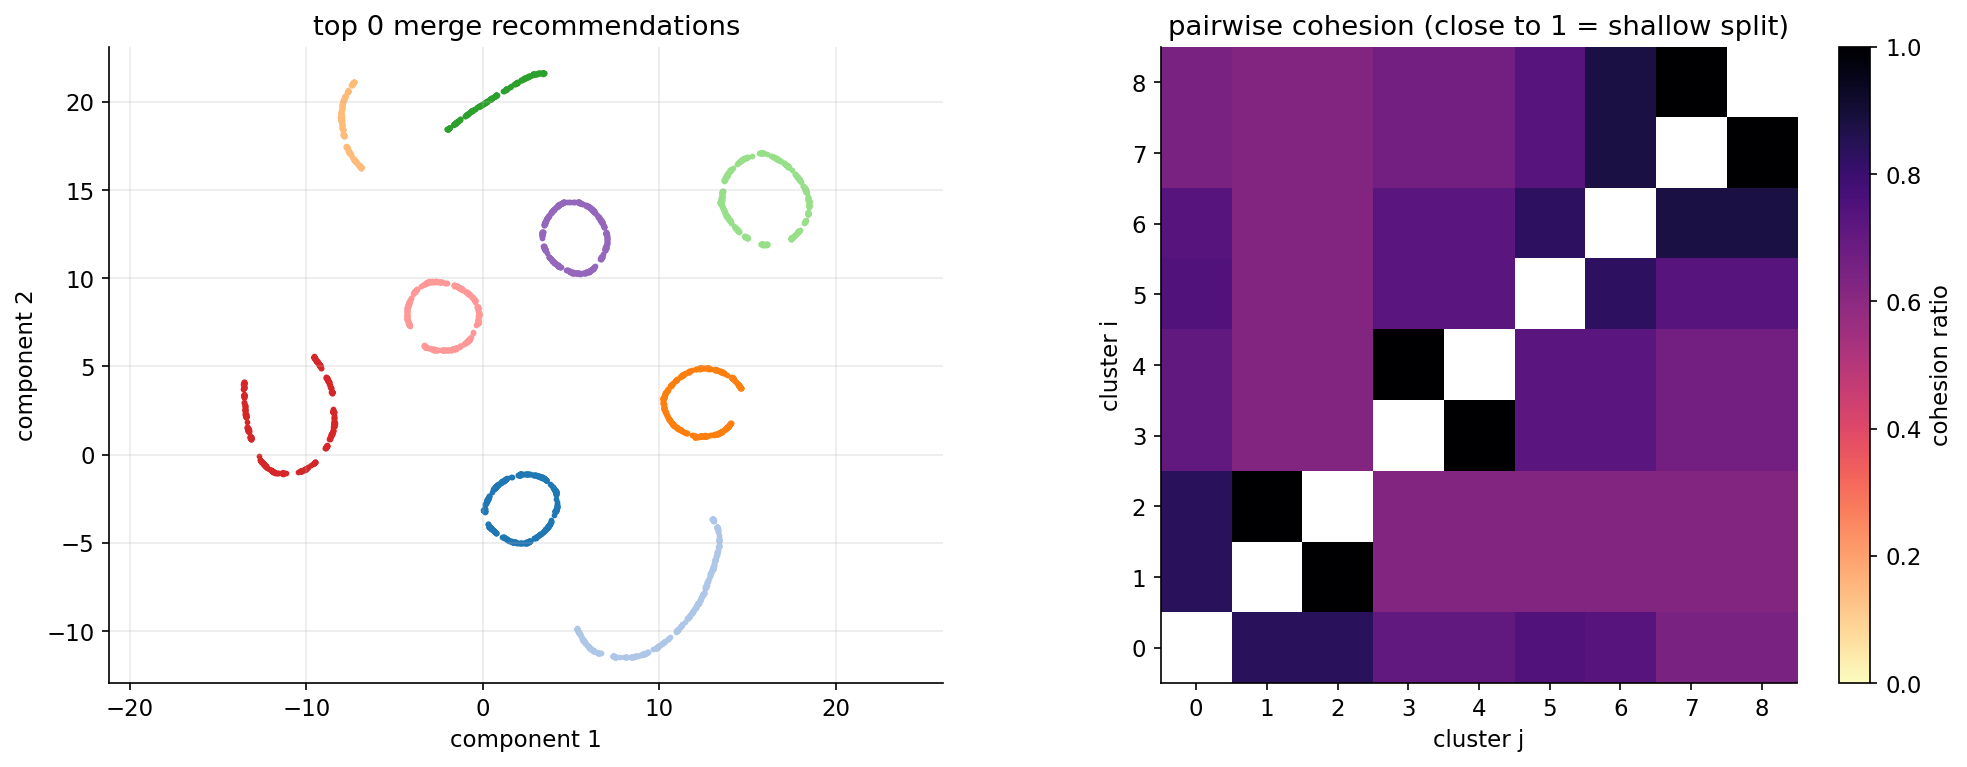
\includegraphics[width=0.85\textwidth]{02_merge_recommendations.png}
  \caption{Merge candidate panel. Each candidate pair is plotted in the (cohesion, gap) plane; recommended pairs sit in the upper-left quadrant. The algorithm does not auto-merge; it surfaces the suggestion for the user to act on.}
  \label{fig:merge-candidates}
\end{figure}

\subsection{Sub-cluster refit}

The paper's second-run workflow (refit on a major component) is a scientific choice, not part of the methodology. \texttt{result.refit\_subcluster(X, cluster\_id)} runs a fresh pipeline on the subset of \(X\) belonging to \texttt{cluster\_id}. The output is another \texttt{PipelineResult}, with its own embedding, labels, persistence, and noise baseline.

\subsection{Robustness diagnostics}
\label{sec:robustness}

\paragraph{Chunked silhouette.} The classical silhouette computation builds an \(N \times N\) distance matrix and is prohibitive at \(N > 10^4\). \texttt{chunked\_silhouette} computes per-cluster aggregates in chunks of \texttt{chunk\_size=512} samples by default, keeping peak memory at \(\mathcal{O}(N \cdot \texttt{chunk\_size})\). \Cref{fig:silhouette} shows the per-cluster silhouette breakdown.

\begin{figure}[h]
  \centering
  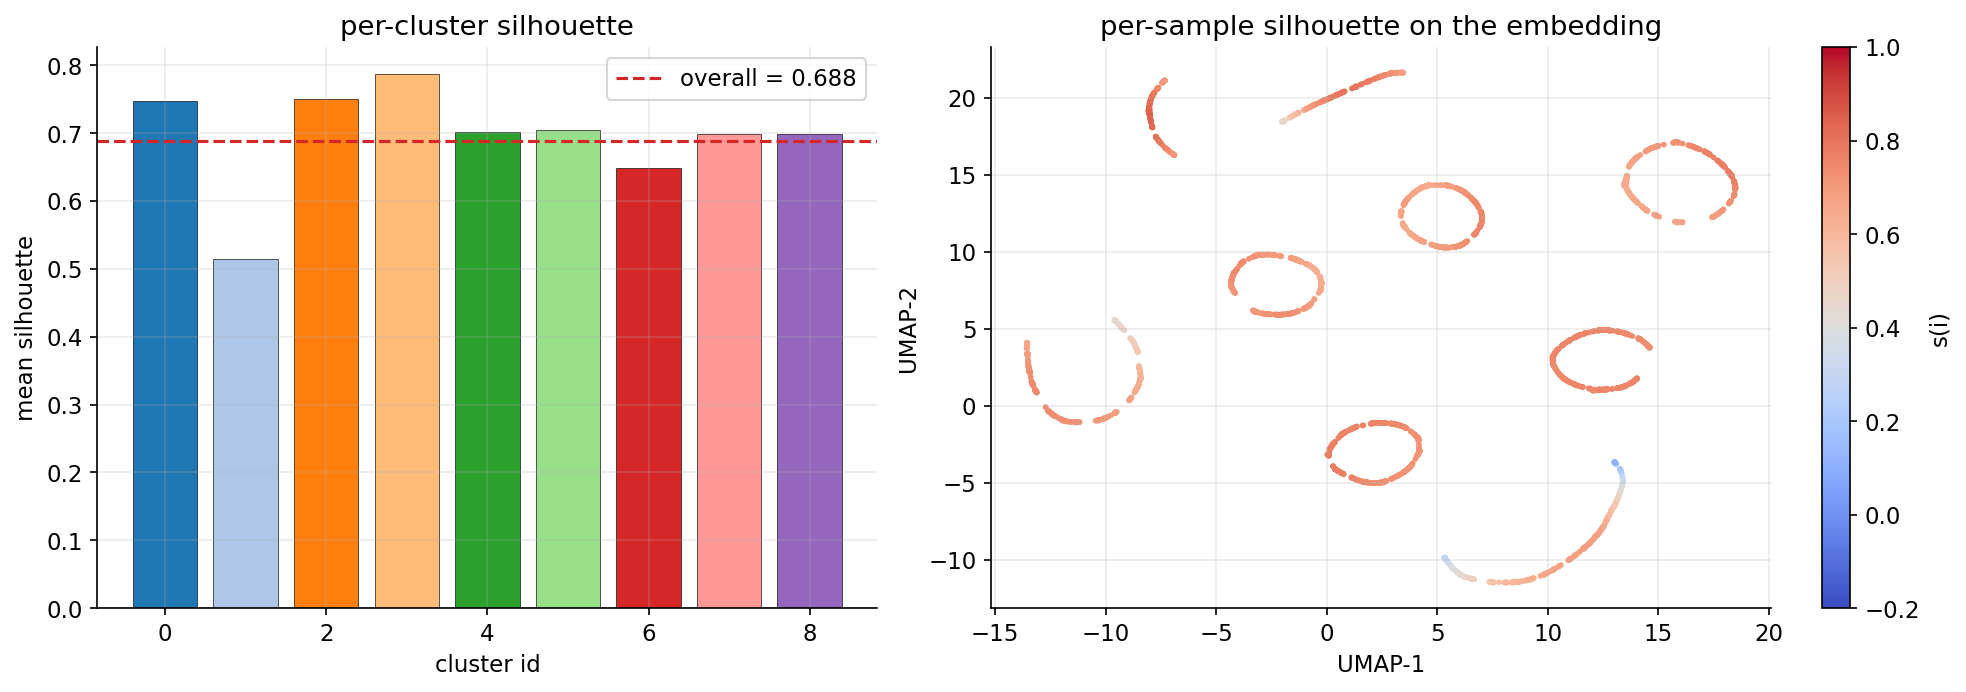
\includegraphics[width=0.7\textwidth]{01_silhouette.png}
  \caption{Per-cluster silhouette and overall score. Bars below zero indicate clusters whose internal cohesion is worse than their separation from the nearest neighbour cluster, a candidate for refinement.}
  \label{fig:silhouette}
\end{figure}

\paragraph{Subsample stability.} \texttt{compute\_subsample\_stability} resamples the embedding (default 20 subsamples at 80\% fraction), refits HDBSCAN on each, aligns labels via the Hungarian algorithm against the reference fit, and reports the distribution of adjusted Rand index (ARI). A high-mean low-variance ARI distribution is the strongest single signal that the clustering is reproducible under data perturbation.

% =========================================================================
\section{Plotting: two single-call dashboards}
\label{sec:dashboards}

\textsf{starfold} exposes seven composable plot primitives and bundles the most diagnostic of them into two single-call dashboards on \texttt{PipelineResult}.

\subsection{Tuning dashboard}

\texttt{result.plot\_tuning\_dashboard()} renders eight panels covering the Optuna search:
\begin{itemize}[leftmargin=*,nosep]
  \item optimisation history (best value vs trial),
  \item parameter importance (fANOVA),
  \item the 2-D \((\texttt{min\_cluster\_size}, \texttt{min\_samples})\) landscape,
  \item the condensed tree of the final fit,
  \item the per-cluster persistence bar chart,
  \item the (objective vs trial) parallel coordinates plot,
  \item the granularity stability sweep,
  \item the trustworthiness curve over \(k\).
\end{itemize}
\Cref{fig:tuning-dashboard} shows the full assembly.

\begin{figure}[h]
  \centering
  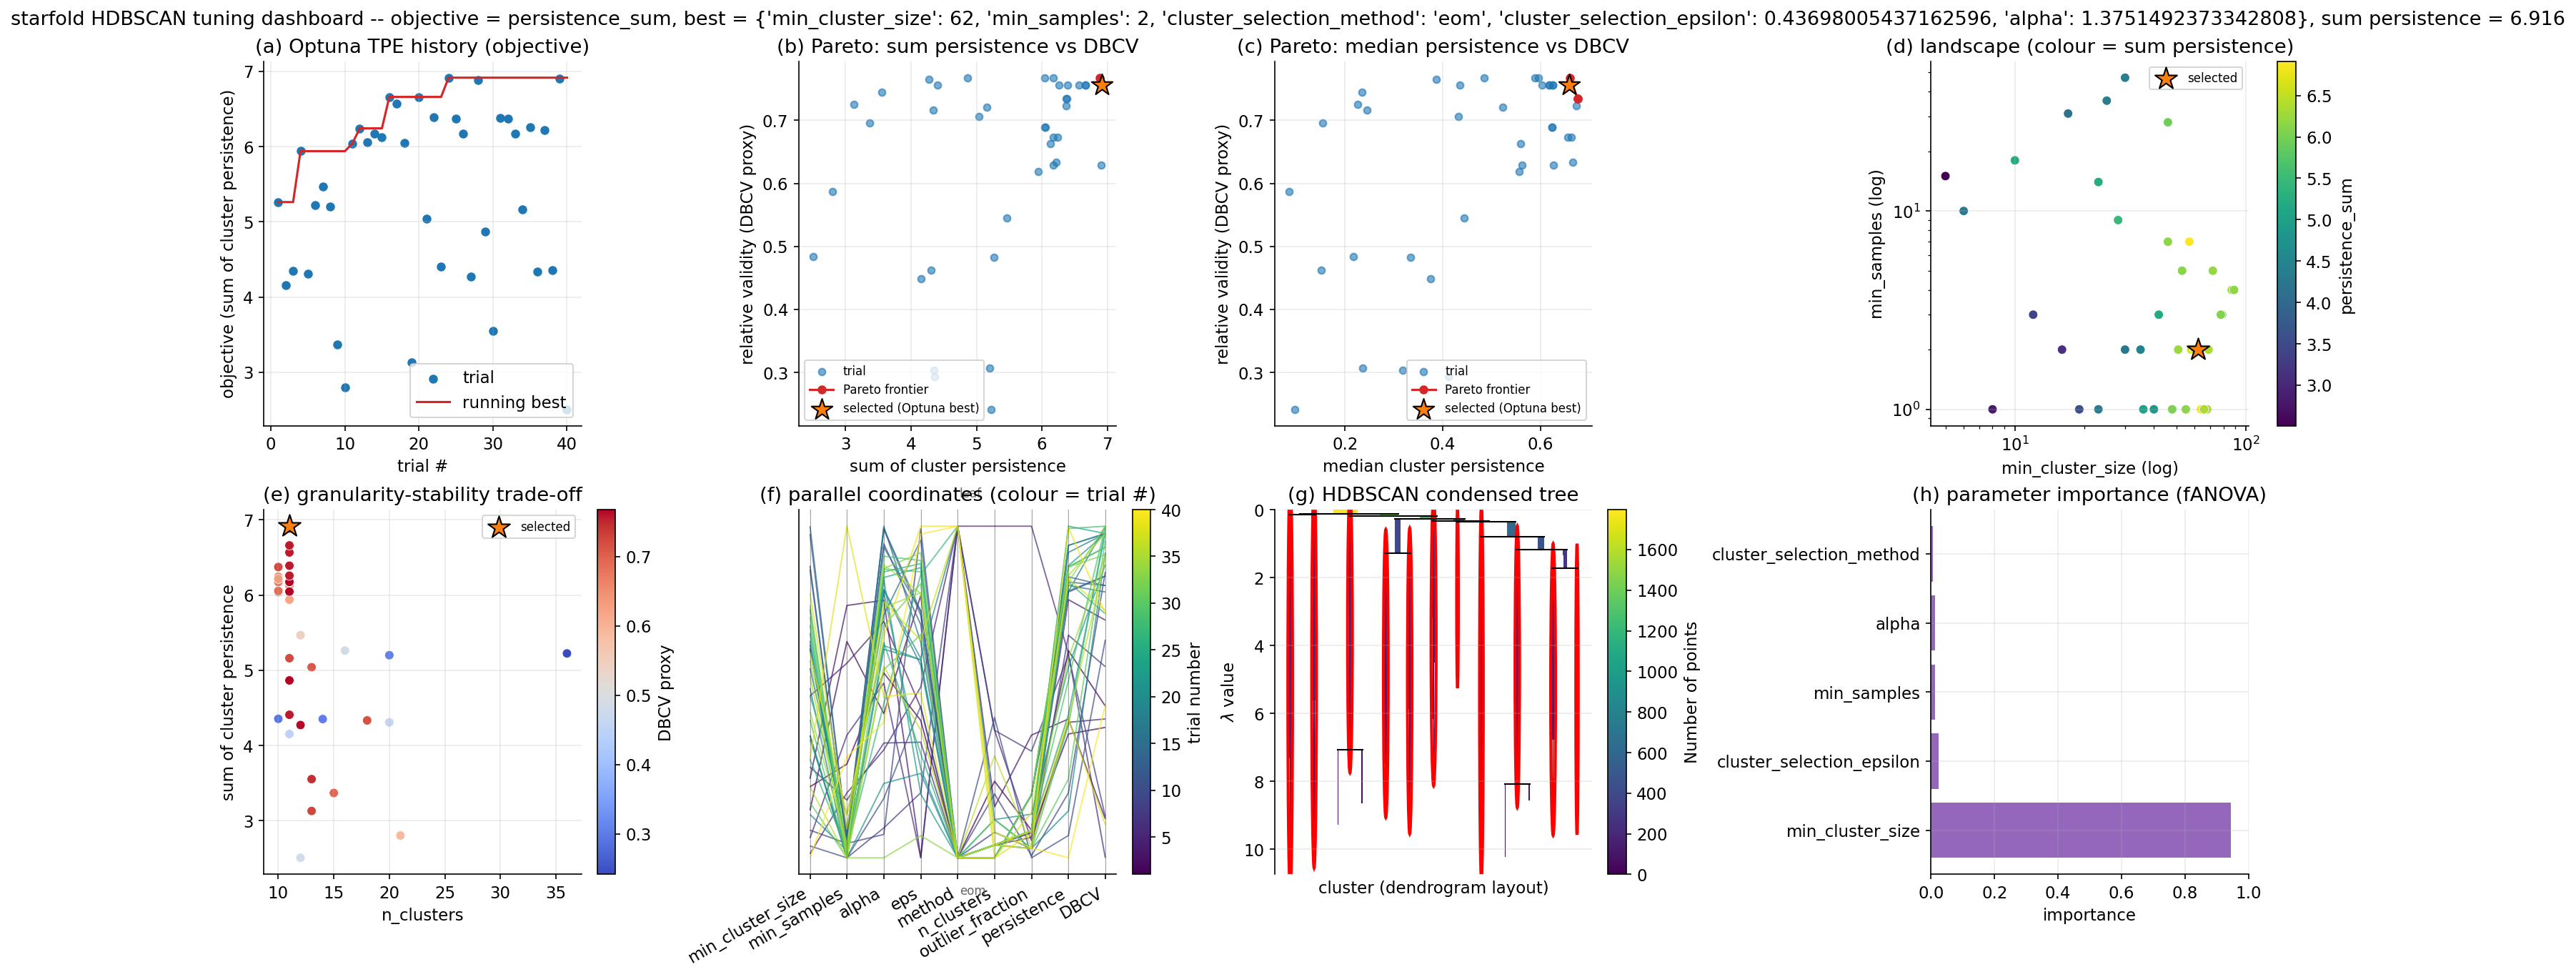
\includegraphics[width=\textwidth]{08_tuning_dashboard.png}
  \caption{The tuning dashboard. Eight panels on one canvas summarise the Optuna search and the structure of the HDBSCAN fit it selected.}
  \label{fig:tuning-dashboard}
\end{figure}

\subsection{Quality dashboard}

\texttt{result.plot\_quality\_dashboard(X)} renders six panels covering the fitted model:
\begin{itemize}[leftmargin=*,nosep]
  \item membership confidence (when an uncertainty propagation has been attached),
  \item Optuna fANOVA importance for the final search,
  \item trustworthiness and continuity curves over \(k\),
  \item subsample stability summary (ARI distribution),
  \item ARI vs subsample, and
  \item cluster-count vs subsample.
\end{itemize}
\Cref{fig:quality-dashboard} shows the full assembly.

\begin{figure}[h]
  \centering
  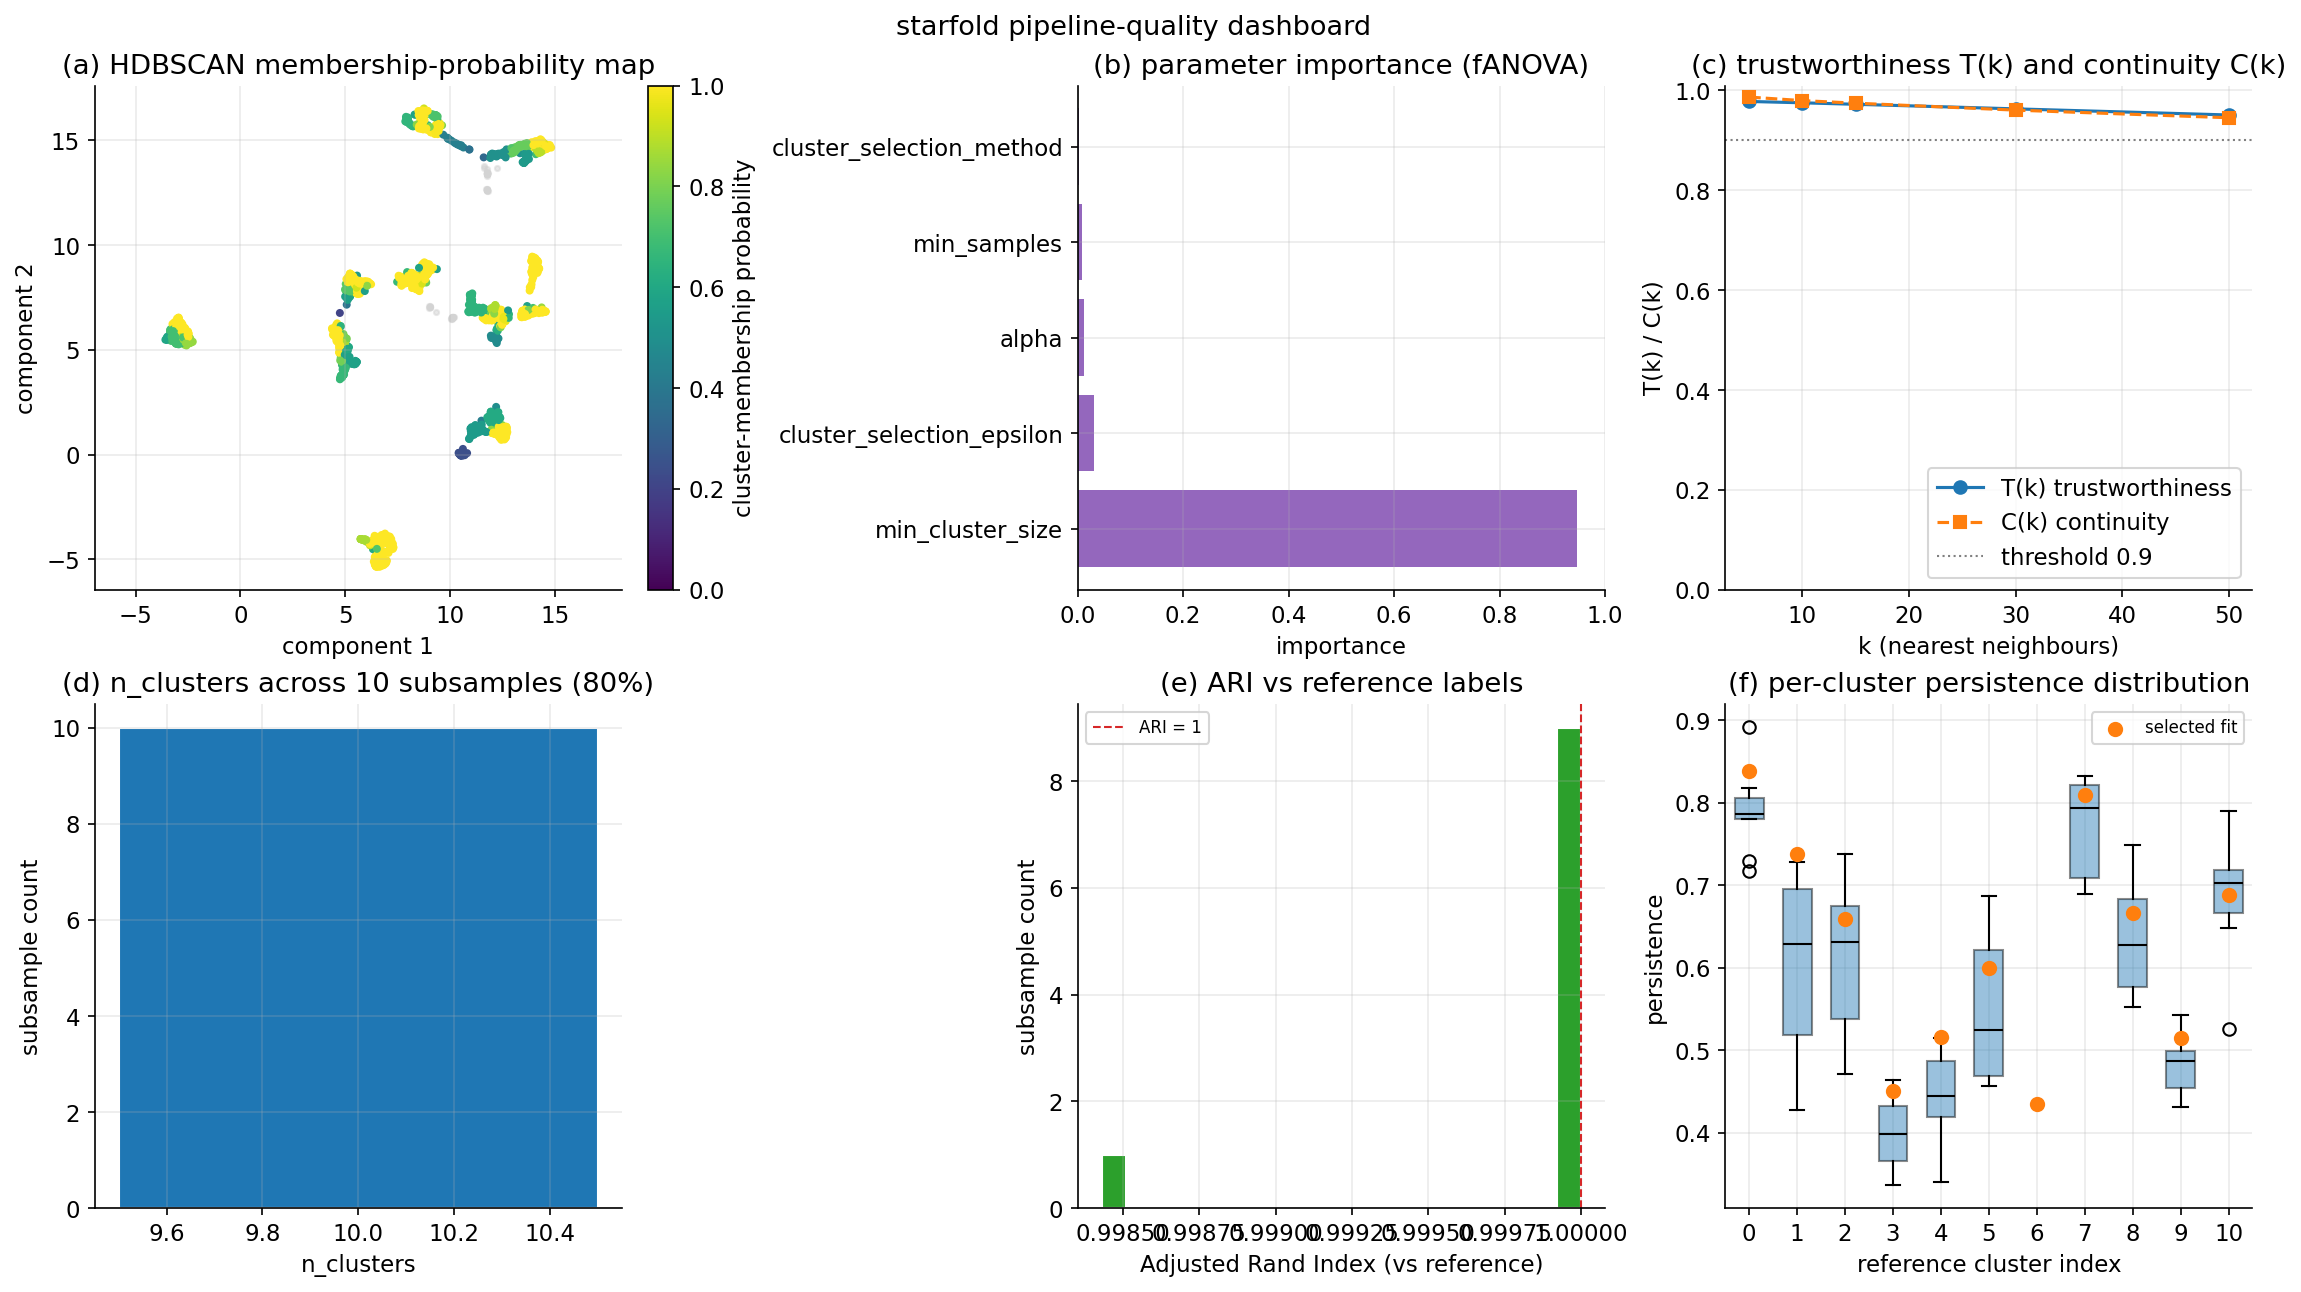
\includegraphics[width=\textwidth]{09_quality_dashboard.png}
  \caption{The quality dashboard. Six panels validate the final fit: membership confidence, parameter importance, embedding fidelity, and stability under resampling.}
  \label{fig:quality-dashboard}
\end{figure}

% =========================================================================
\section{Refinement workflow}

A typical workflow after a clean fit:
\begin{enumerate}[leftmargin=*,nosep]
  \item Inspect \texttt{result.summary()} and the tuning dashboard. Were the chosen hyperparameters at the boundary of the search range?
  \item Run \texttt{result.silhouette()} and the quality dashboard. Are any clusters below silhouette \(0\)?
  \item Inspect \texttt{result.suggest\_merges()}. Are there cohesive, geometrically-close pairs?
  \item If so, decide whether to merge (or to inspect data-domain centroids first).
\end{enumerate}

\Cref{fig:before-after} compares a baseline fit against two refinement strategies on the digits dataset: ``blind'' (merge the algorithm's top suggestion) versus ``inspection-informed'' (look at cluster centroids and merge two clusters that both look like the digit ``1''). The inspection-informed strategy improves ARI from \num{0.870} to \num{0.891}; the blind strategy degrades it. The recommendation flag agrees: the blind pair had \texttt{recommended=False}.

\begin{figure}[h]
  \centering
  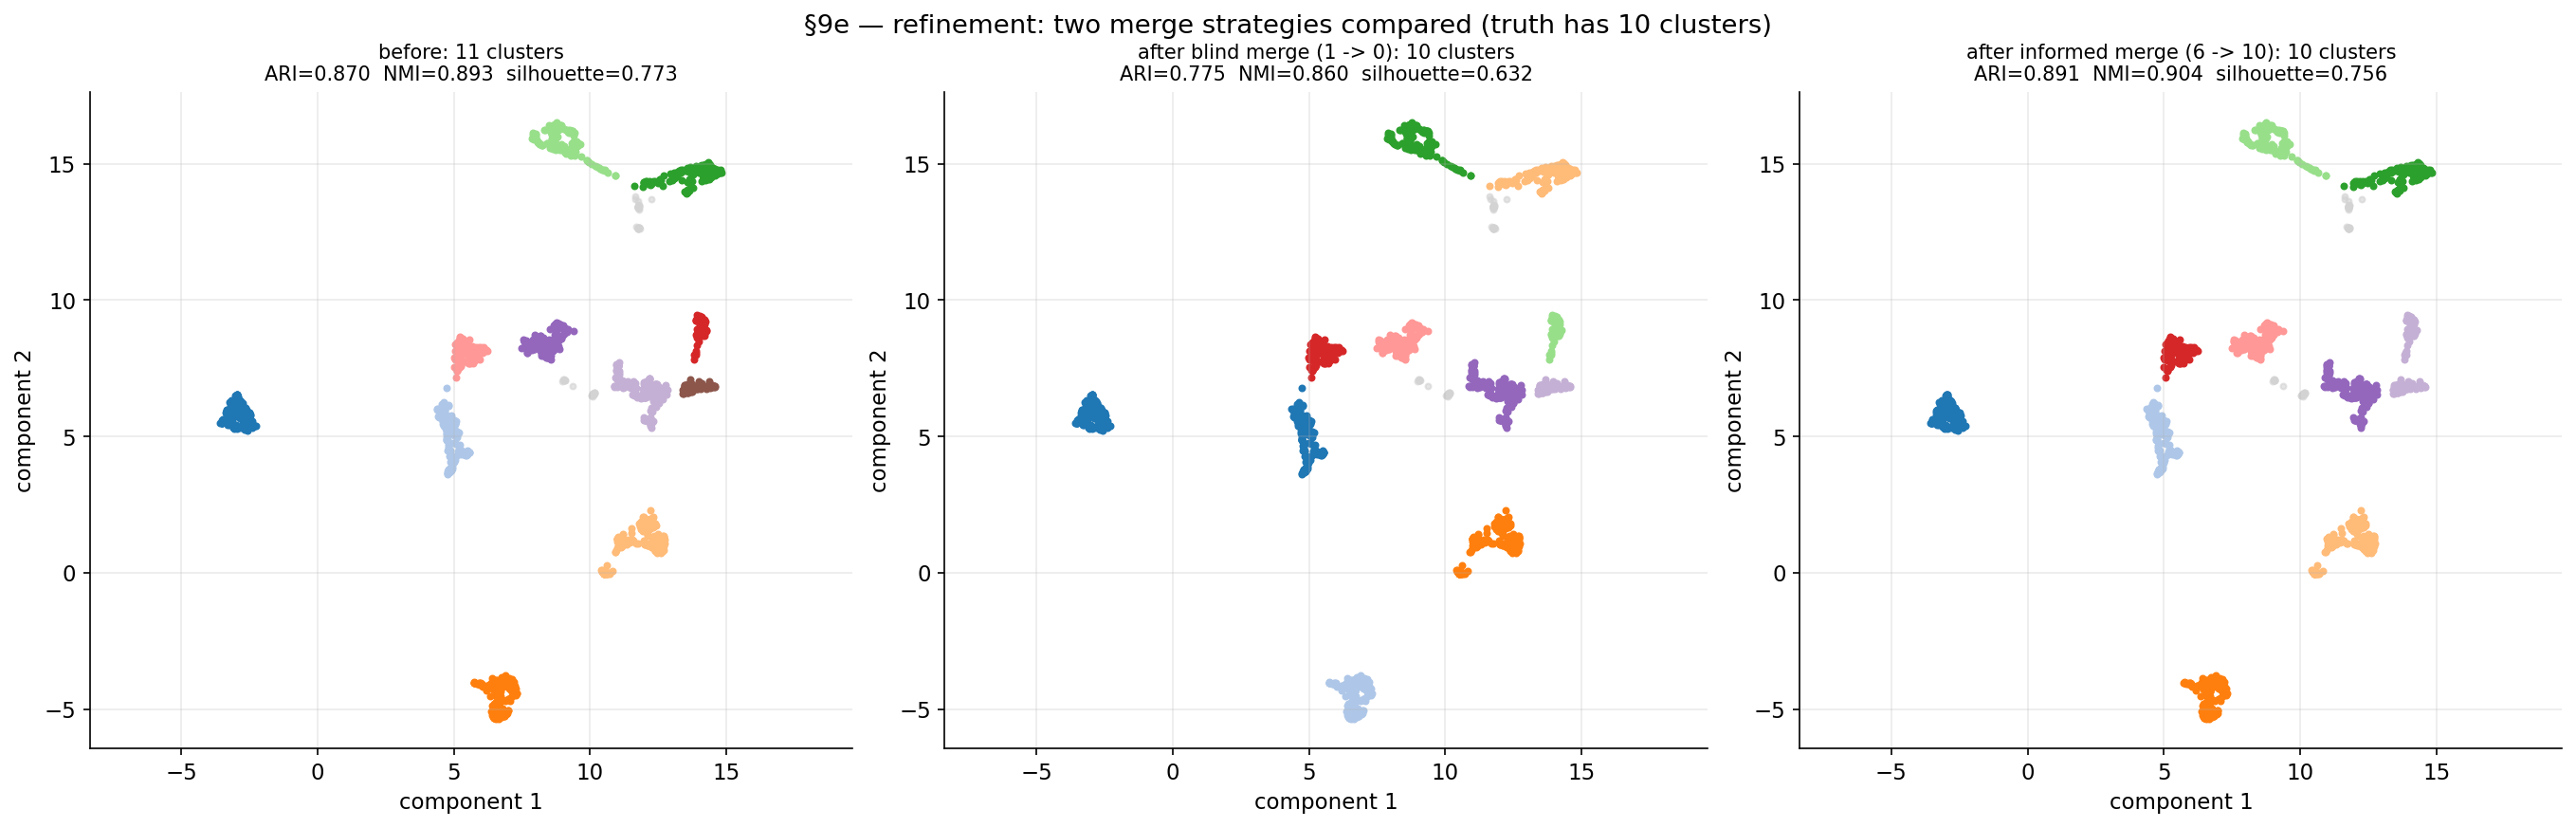
\includegraphics[width=\textwidth]{11_before_after_refinement.png}
  \caption{Refinement comparison on \texttt{sklearn.datasets.load\_digits}. Left: clean fit (ARI \num{0.870}). Centre: blind merge of the top \texttt{suggest\_merges} candidate (ARI \num{0.775}, degrades). Right: inspection-informed merge of two clusters whose centroid images both look like the digit ``1'' (ARI \num{0.891}, improves).}
  \label{fig:before-after}
\end{figure}

% =========================================================================
\section{Persistence and reproducibility}

\subsection{Save and reload}

\texttt{result.save(directory)} writes the embedding, labels, persistence, trustworthiness, fitted scaler and UMAP reducer, run configuration, noise-baseline summary, and credibility report into a directory. \texttt{sf.load\_pipeline\_result(directory)} returns the same content as a plain dict; the Optuna study is not rehydrated (it is stored only as a JSON summary). The numerical-array round-trip is bit-faithful, so a saved fit is the canonical archive of a clustering run.

\begin{pycode}
result.save("runs/run_01/")
loaded = sf.load_pipeline_result("runs/run_01/")
assert np.array_equal(loaded["labels"], result.labels)
\end{pycode}

\subsection{Determinism}

Every stochastic call accepts a \texttt{random\_state} that propagates to UMAP, the Optuna TPE sampler, the noise-baseline noise generator, and the uncertainty Monte Carlo. With a fixed seed, results are bit-reproducible across runs on the same machine.

% =========================================================================
\section{Public API surface (30 symbols)}
\label{sec:api}

\textsf{starfold}'s public API, exported from \texttt{starfold/\_\_init\_\_.py}:

\begin{table}[h]
  \centering
  \footnotesize
  \begin{tabular}{p{0.30\textwidth} p{0.62\textwidth}}
    \toprule
    Symbol & Role \\
    \midrule
    \multicolumn{2}{l}{\textbf{Core entry points}} \\
    \texttt{UnsupervisedPipeline} & The pipeline object; one method, \texttt{.fit(X)}. \\
    \texttt{PipelineResult} & Immutable audit trail of a fit. \\
    \midrule
    \multicolumn{2}{l}{\textbf{Core building blocks}} \\
    \texttt{run\_umap}, \texttt{run\_tsne}, \texttt{run\_pca} & Embedding wrappers (UMAP is canonical). \\
    \texttt{trustworthiness}, \texttt{continuity} & Single-\(k\) scores. \\
    \texttt{trustworthiness\_curve}, \texttt{continuity\_curve} & Multi-\(k\) curves. \\
    \texttt{run\_hdbscan} & Single HDBSCAN fit at fixed hyperparameters. \\
    \texttt{search\_hdbscan} & Optuna-tuned HDBSCAN. \\
    \texttt{compute\_noise\_baseline} & 99.7th-percentile baseline (cached). \\
    \midrule
    \multicolumn{2}{l}{\textbf{Extension primitives}} \\
    \texttt{compute\_credibility} & Omnibus 3-sigma test. \\
    \texttt{propagate\_uncertainty} & Post-hoc Monte Carlo on a frozen fit. \\
    \texttt{suggest\_merges} & Hierarchical merge recommender. \\
    \texttt{chunked\_silhouette} & Memory-efficient silhouette. \\
    \texttt{compute\_subsample\_stability} & Bootstrap-like ARI distribution. \\
    \midrule
    \multicolumn{2}{l}{\textbf{Plot helpers}} \\
    \texttt{plot\_embedding}, \texttt{plot\_embedding\_comparison} & Scatter plots and side-by-sides. \\
    \texttt{plot\_trustworthiness\_curve} & T(k) and C(k) line plot. \\
    \texttt{plot\_condensed\_tree} & HDBSCAN dendrogram. \\
    \texttt{plot\_optuna\_history}, \texttt{plot\_optuna\_param\_importance} & Optuna diagnostic panels. \\
    \texttt{plot\_uncertainty\_map} & Instability scatter on the embedding. \\
    \midrule
    \multicolumn{2}{l}{\textbf{Utilities}} \\
    \texttt{save\_pipeline\_result}, \texttt{load\_pipeline\_result} & Disk round-trip. \\
    \texttt{validate\_input\_matrix} & Defensive input checks. \\
    \texttt{recommend\_budget}, \texttt{auto\_mcs\_upper} & Sample-size-aware defaults. \\
    \texttt{cuml\_is\_importable} & GPU backend probe. \\
    \bottomrule
  \end{tabular}
\end{table}

% =========================================================================
\section{Applied example: stellar populations}
\label{sec:astronomy}

Tutorial 4 of the bundled notebook arc applies the pipeline to a real chemo-dynamical sample of \num{9242} Milky Way stars from APOGEE DR19 cross-matched with Gaia DR3 and \texttt{galpy}-integrated orbital actions. The package itself has no astronomy dependency; the tutorial uses a pre-built parquet bundled in \texttt{docs/data/}. The fit recovers structure that traces the canonical thin disc, thick disc, and halo populations in the \([\mathrm{Fe/H}], [\alpha/\mathrm{M}]\) chemical plane (\Cref{fig:astro-chem}) and the action space (\Cref{fig:astro-action}), without ever being told about these reference frames.

\begin{figure}[h]
  \centering
  \begin{minipage}{0.48\textwidth}
    \centering
    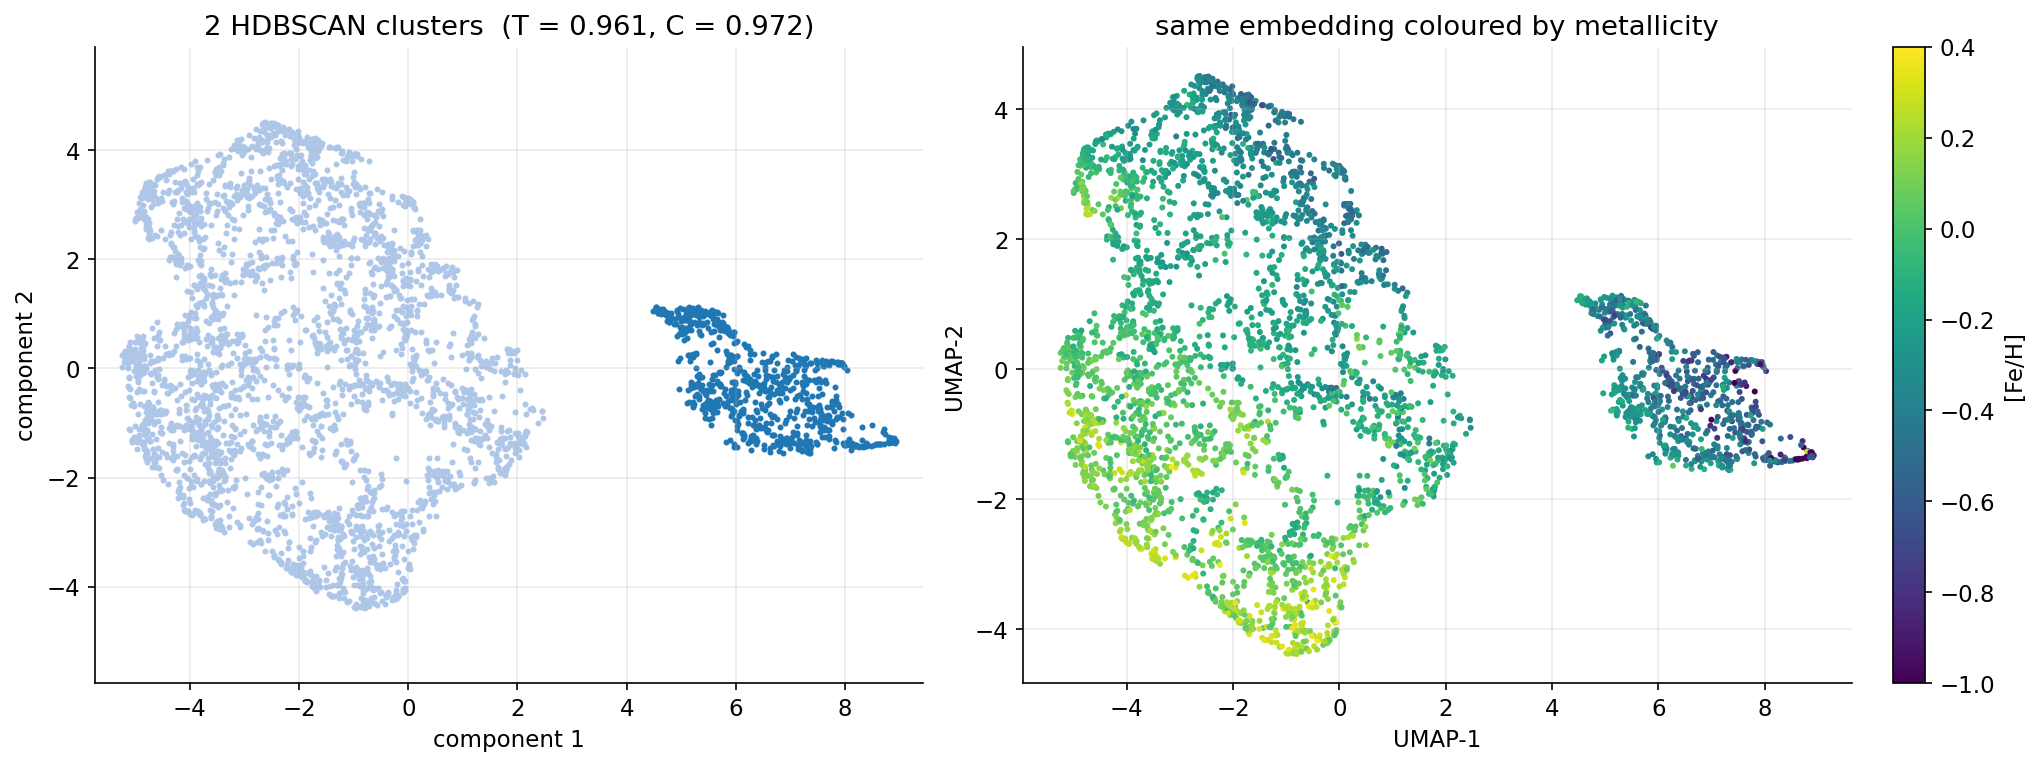
\includegraphics[width=\textwidth]{02_embedding.png}
    \caption{UMAP embedding of \num{9242} stars, coloured by HDBSCAN cluster.}
    \label{fig:astro-embedding}
  \end{minipage}\hfill
  \begin{minipage}{0.48\textwidth}
    \centering
    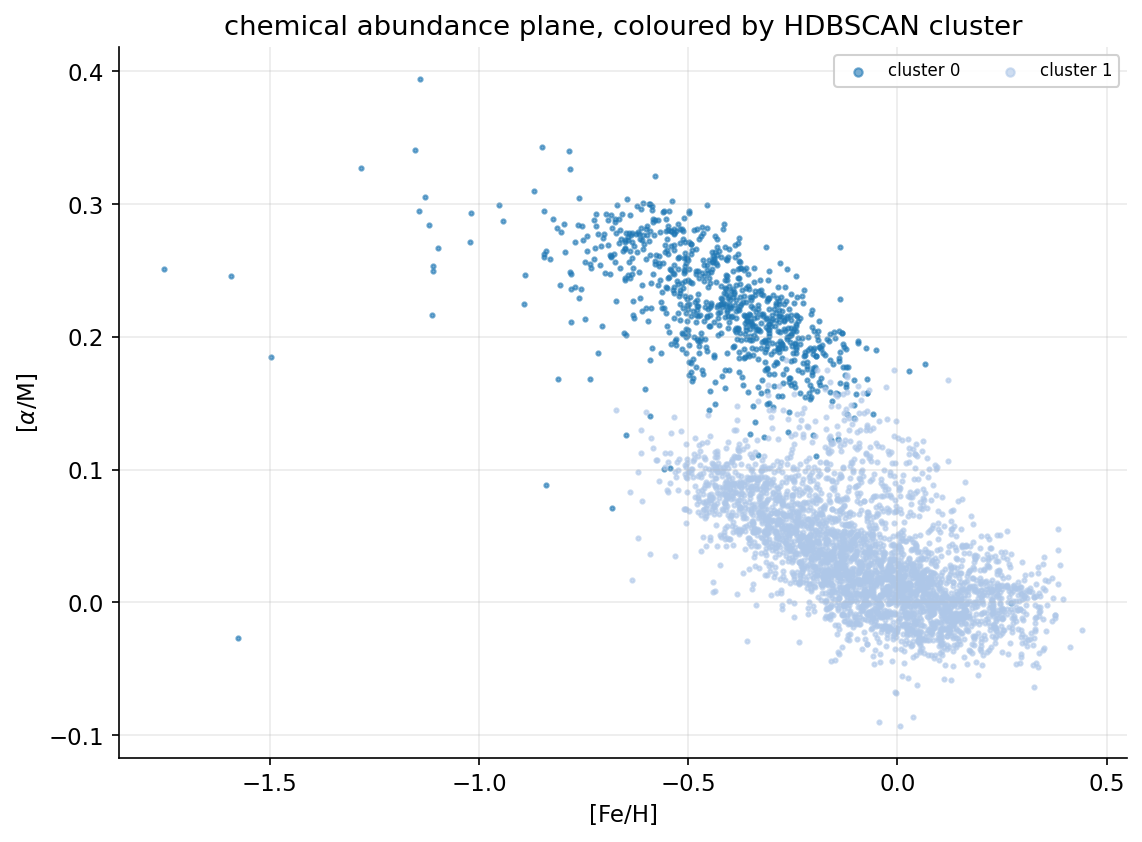
\includegraphics[width=\textwidth]{03_chemical_plane.png}
    \caption{The same clusters projected back onto the chemical plane.}
    \label{fig:astro-chem}
  \end{minipage}
\end{figure}

\begin{figure}[h]
  \centering
  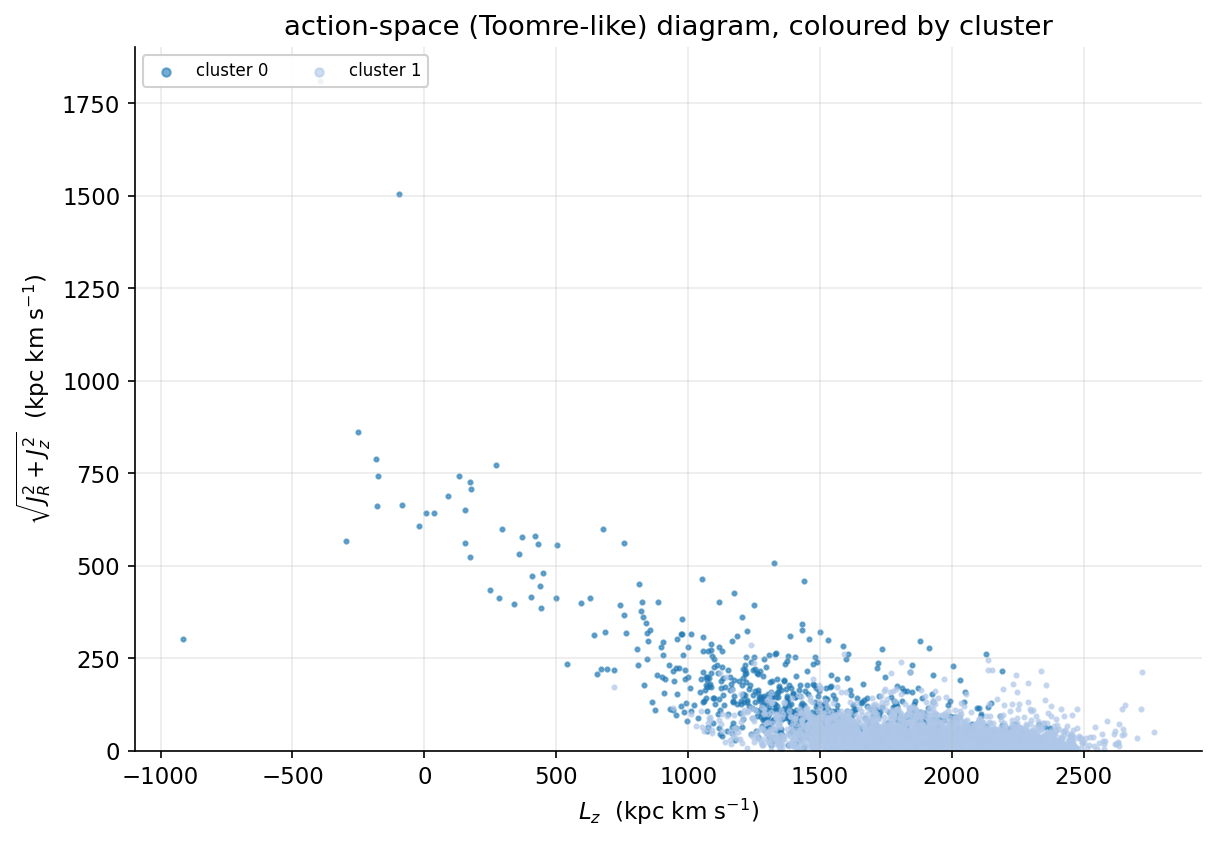
\includegraphics[width=0.7\textwidth]{04_action_space.png}
  \caption{Action-space projection. Disc stars carry circular orbits (low \(J_R^2 + J_z^2\), positive \(L_z\)); halo stars span the rest of the plane.}
  \label{fig:astro-action}
\end{figure}

% =========================================================================
\section{References}

\begin{itemize}[leftmargin=*,nosep]
  \item Neitzel, Campante, Bossini and Miglio (2025). \textit{Astronomy and Astrophysics} \textbf{695}, A243. arXiv:2501.16294.
  \item McInnes, Healy and Melville (2018). UMAP: Uniform Manifold Approximation and Projection. arXiv:1802.03426.
  \item McInnes, Healy and Astels (2017). hdbscan: Hierarchical density-based clustering. \textit{Journal of Open Source Software} \textbf{2}(11), 205.
  \item Venna and Kaski (2001). Neighbourhood preservation in nonlinear projection methods. ICANN 2001.
  \item Akiba et al.\ (2019). Optuna: A next-generation hyperparameter optimization framework. KDD.
  \item Phipson and Smyth (2010). Permutation p-values should never be zero. \textit{Statistical Applications in Genetics and Molecular Biology} \textbf{9}(1).
\end{itemize}

\vspace{1em}
\noindent
\textbf{Citation.} If you use \textsf{starfold} in published research, please cite the parent paper (Neitzel et al.\ 2025) and the software via \texttt{CITATION.cff}.

\end{document}
